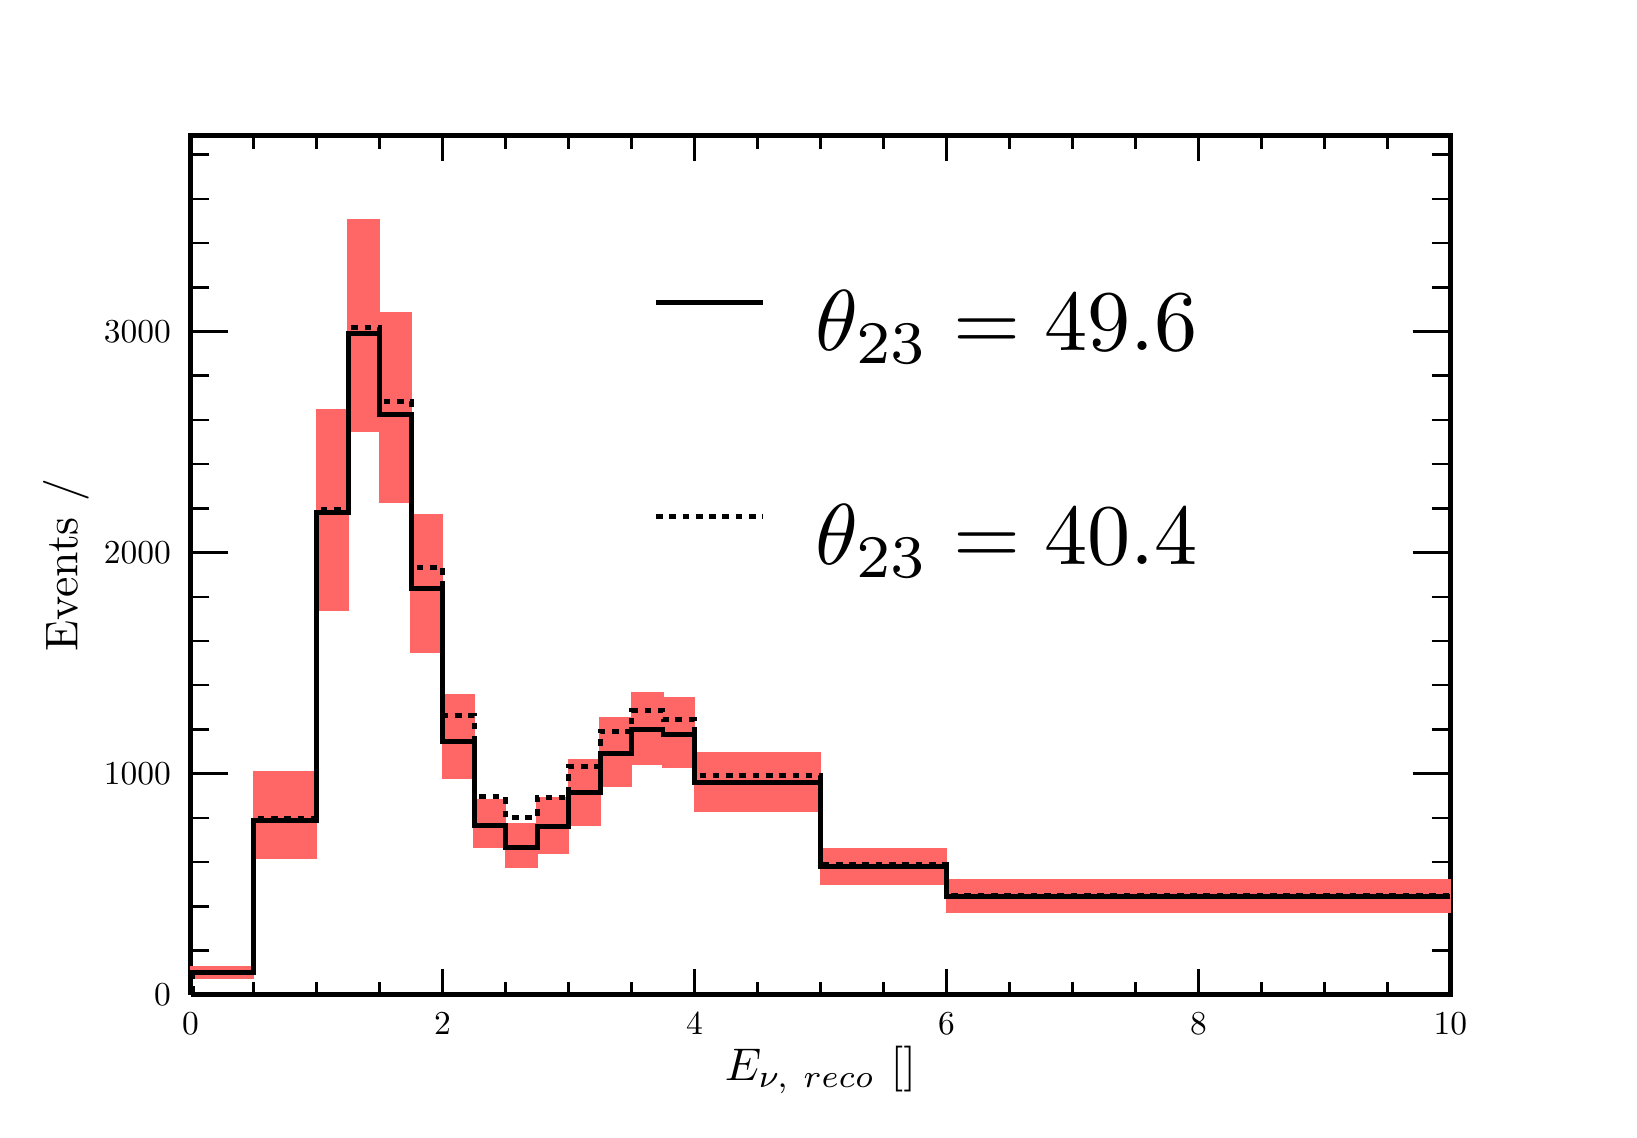
\begin{tikzpicture}
\pgfdeclareplotmark{cross} {
\pgfpathmoveto{\pgfpoint{-0.3\pgfplotmarksize}{\pgfplotmarksize}}
\pgfpathlineto{\pgfpoint{+0.3\pgfplotmarksize}{\pgfplotmarksize}}
\pgfpathlineto{\pgfpoint{+0.3\pgfplotmarksize}{0.3\pgfplotmarksize}}
\pgfpathlineto{\pgfpoint{+1\pgfplotmarksize}{0.3\pgfplotmarksize}}
\pgfpathlineto{\pgfpoint{+1\pgfplotmarksize}{-0.3\pgfplotmarksize}}
\pgfpathlineto{\pgfpoint{+0.3\pgfplotmarksize}{-0.3\pgfplotmarksize}}
\pgfpathlineto{\pgfpoint{+0.3\pgfplotmarksize}{-1.\pgfplotmarksize}}
\pgfpathlineto{\pgfpoint{-0.3\pgfplotmarksize}{-1.\pgfplotmarksize}}
\pgfpathlineto{\pgfpoint{-0.3\pgfplotmarksize}{-0.3\pgfplotmarksize}}
\pgfpathlineto{\pgfpoint{-1.\pgfplotmarksize}{-0.3\pgfplotmarksize}}
\pgfpathlineto{\pgfpoint{-1.\pgfplotmarksize}{0.3\pgfplotmarksize}}
\pgfpathlineto{\pgfpoint{-0.3\pgfplotmarksize}{0.3\pgfplotmarksize}}
\pgfpathclose
\pgfusepathqstroke
}
\pgfdeclareplotmark{cross*} {
\pgfpathmoveto{\pgfpoint{-0.3\pgfplotmarksize}{\pgfplotmarksize}}
\pgfpathlineto{\pgfpoint{+0.3\pgfplotmarksize}{\pgfplotmarksize}}
\pgfpathlineto{\pgfpoint{+0.3\pgfplotmarksize}{0.3\pgfplotmarksize}}
\pgfpathlineto{\pgfpoint{+1\pgfplotmarksize}{0.3\pgfplotmarksize}}
\pgfpathlineto{\pgfpoint{+1\pgfplotmarksize}{-0.3\pgfplotmarksize}}
\pgfpathlineto{\pgfpoint{+0.3\pgfplotmarksize}{-0.3\pgfplotmarksize}}
\pgfpathlineto{\pgfpoint{+0.3\pgfplotmarksize}{-1.\pgfplotmarksize}}
\pgfpathlineto{\pgfpoint{-0.3\pgfplotmarksize}{-1.\pgfplotmarksize}}
\pgfpathlineto{\pgfpoint{-0.3\pgfplotmarksize}{-0.3\pgfplotmarksize}}
\pgfpathlineto{\pgfpoint{-1.\pgfplotmarksize}{-0.3\pgfplotmarksize}}
\pgfpathlineto{\pgfpoint{-1.\pgfplotmarksize}{0.3\pgfplotmarksize}}
\pgfpathlineto{\pgfpoint{-0.3\pgfplotmarksize}{0.3\pgfplotmarksize}}
\pgfpathclose
\pgfusepathqfillstroke
}
\pgfdeclareplotmark{newstar} {
\pgfpathmoveto{\pgfqpoint{0pt}{\pgfplotmarksize}}
\pgfpathlineto{\pgfqpointpolar{44}{0.5\pgfplotmarksize}}
\pgfpathlineto{\pgfqpointpolar{18}{\pgfplotmarksize}}
\pgfpathlineto{\pgfqpointpolar{-20}{0.5\pgfplotmarksize}}
\pgfpathlineto{\pgfqpointpolar{-54}{\pgfplotmarksize}}
\pgfpathlineto{\pgfqpointpolar{-90}{0.5\pgfplotmarksize}}
\pgfpathlineto{\pgfqpointpolar{234}{\pgfplotmarksize}}
\pgfpathlineto{\pgfqpointpolar{198}{0.5\pgfplotmarksize}}
\pgfpathlineto{\pgfqpointpolar{162}{\pgfplotmarksize}}
\pgfpathlineto{\pgfqpointpolar{134}{0.5\pgfplotmarksize}}
\pgfpathclose
\pgfusepathqstroke
}
\pgfdeclareplotmark{newstar*} {
\pgfpathmoveto{\pgfqpoint{0pt}{\pgfplotmarksize}}
\pgfpathlineto{\pgfqpointpolar{44}{0.5\pgfplotmarksize}}
\pgfpathlineto{\pgfqpointpolar{18}{\pgfplotmarksize}}
\pgfpathlineto{\pgfqpointpolar{-20}{0.5\pgfplotmarksize}}
\pgfpathlineto{\pgfqpointpolar{-54}{\pgfplotmarksize}}
\pgfpathlineto{\pgfqpointpolar{-90}{0.5\pgfplotmarksize}}
\pgfpathlineto{\pgfqpointpolar{234}{\pgfplotmarksize}}
\pgfpathlineto{\pgfqpointpolar{198}{0.5\pgfplotmarksize}}
\pgfpathlineto{\pgfqpointpolar{162}{\pgfplotmarksize}}
\pgfpathlineto{\pgfqpointpolar{134}{0.5\pgfplotmarksize}}
\pgfpathclose
\pgfusepathqfillstroke
}
\definecolor{c}{rgb}{0.999,0.999,0.999};
\draw [color=c, fill=c] (0,0) rectangle (20,13.639);
\draw [color=c, fill=c] (2,1.3639) rectangle (18,12.2751);
\definecolor{c}{rgb}{0,0,0};
\draw [c,line width=1.8] (2,1.3639) -- (2,12.2751) -- (18,12.2751) -- (18,1.3639) -- (2,1.3639);
\definecolor{c}{rgb}{0.999,0.999,0.999};
\draw [color=c, fill=c] (2,1.3639) rectangle (18,12.2751);
\definecolor{c}{rgb}{0,0,0};
\draw [c,line width=1.8] (2,1.3639) -- (2,12.2751) -- (18,12.2751) -- (18,1.3639) -- (2,1.3639);
\draw [c,line width=1.8] (2,1.64499) -- (2.8,1.64499) -- (2.8,3.58066) -- (3.6,3.58066) -- (3.6,7.48952) -- (4,7.48952) -- (4,9.75711) -- (4.4,9.75711) -- (4.4,8.72912) -- (4.8,8.72912) -- (4.8,6.52389) -- (5.2,6.52389) -- (5.2,4.58459) --
 (5.6,4.58459) -- (5.6,3.51089) -- (6,3.51089) -- (6,3.23684) -- (6.4,3.23684) -- (6.4,3.5047) -- (6.8,3.5047) -- (6.8,3.93032) -- (7.2,3.93032) -- (7.2,4.42465) -- (7.6,4.42465) -- (7.6,4.73254) -- (8,4.73254) -- (8,4.6717) -- (8.4,4.6717) --
 (8.4,4.05577) -- (10,4.05577) -- (10,2.98825) -- (11.6,2.98825) -- (11.6,2.61432) -- (18,2.61432);
\draw [c,line width=0.9] (2,1.3639) -- (18,1.3639);
\draw [c,line width=0.9] (2,1.69123) -- (2,1.3639);
\draw [c,line width=0.9] (2.8,1.52756) -- (2.8,1.3639);
\draw [c,line width=0.9] (3.6,1.52756) -- (3.6,1.3639);
\draw [c,line width=0.9] (4.4,1.52756) -- (4.4,1.3639);
\draw [c,line width=0.9] (5.2,1.69123) -- (5.2,1.3639);
\draw [c,line width=0.9] (6,1.52756) -- (6,1.3639);
\draw [c,line width=0.9] (6.8,1.52756) -- (6.8,1.3639);
\draw [c,line width=0.9] (7.6,1.52756) -- (7.6,1.3639);
\draw [c,line width=0.9] (8.4,1.69123) -- (8.4,1.3639);
\draw [c,line width=0.9] (9.2,1.52756) -- (9.2,1.3639);
\draw [c,line width=0.9] (10,1.52756) -- (10,1.3639);
\draw [c,line width=0.9] (10.8,1.52756) -- (10.8,1.3639);
\draw [c,line width=0.9] (11.6,1.69123) -- (11.6,1.3639);
\draw [c,line width=0.9] (12.4,1.52756) -- (12.4,1.3639);
\draw [c,line width=0.9] (13.2,1.52756) -- (13.2,1.3639);
\draw [c,line width=0.9] (14,1.52756) -- (14,1.3639);
\draw [c,line width=0.9] (14.8,1.69123) -- (14.8,1.3639);
\draw [c,line width=0.9] (15.6,1.52756) -- (15.6,1.3639);
\draw [c,line width=0.9] (16.4,1.52756) -- (16.4,1.3639);
\draw [c,line width=0.9] (17.2,1.52756) -- (17.2,1.3639);
\draw [c,line width=0.9] (18,1.69123) -- (18,1.3639);
\draw [anchor=base] (2,0.859255) node[scale=1.20912, color=c, rotate=0]{0};
\draw [anchor=base] (5.2,0.859255) node[scale=1.20912, color=c, rotate=0]{2};
\draw [anchor=base] (8.4,0.859255) node[scale=1.20912, color=c, rotate=0]{4};
\draw [anchor=base] (11.6,0.859255) node[scale=1.20912, color=c, rotate=0]{6};
\draw [anchor=base] (14.8,0.859255) node[scale=1.20912, color=c, rotate=0]{8};
\draw [anchor=base] (18,0.859255) node[scale=1.20912, color=c, rotate=0]{10};
\draw (10,0.403714) node[scale=1.65459, color=c, rotate=0]{$E_{\nu,~\text{reco}}$ [\si{\GeV}]};
\draw [c,line width=0.9] (2,12.2751) -- (18,12.2751);
\draw [c,line width=0.9] (2,11.9477) -- (2,12.2751);
\draw [c,line width=0.9] (2.8,12.1114) -- (2.8,12.2751);
\draw [c,line width=0.9] (3.6,12.1114) -- (3.6,12.2751);
\draw [c,line width=0.9] (4.4,12.1114) -- (4.4,12.2751);
\draw [c,line width=0.9] (5.2,11.9477) -- (5.2,12.2751);
\draw [c,line width=0.9] (6,12.1114) -- (6,12.2751);
\draw [c,line width=0.9] (6.8,12.1114) -- (6.8,12.2751);
\draw [c,line width=0.9] (7.6,12.1114) -- (7.6,12.2751);
\draw [c,line width=0.9] (8.4,11.9477) -- (8.4,12.2751);
\draw [c,line width=0.9] (9.2,12.1114) -- (9.2,12.2751);
\draw [c,line width=0.9] (10,12.1114) -- (10,12.2751);
\draw [c,line width=0.9] (10.8,12.1114) -- (10.8,12.2751);
\draw [c,line width=0.9] (11.6,11.9477) -- (11.6,12.2751);
\draw [c,line width=0.9] (12.4,12.1114) -- (12.4,12.2751);
\draw [c,line width=0.9] (13.2,12.1114) -- (13.2,12.2751);
\draw [c,line width=0.9] (14,12.1114) -- (14,12.2751);
\draw [c,line width=0.9] (14.8,11.9477) -- (14.8,12.2751);
\draw [c,line width=0.9] (15.6,12.1114) -- (15.6,12.2751);
\draw [c,line width=0.9] (16.4,12.1114) -- (16.4,12.2751);
\draw [c,line width=0.9] (17.2,12.1114) -- (17.2,12.2751);
\draw [c,line width=0.9] (18,11.9477) -- (18,12.2751);
\draw [c,line width=0.9] (2,1.3639) -- (2,12.2751);
\draw [c,line width=0.9] (2.48,1.3639) -- (2,1.3639);
\draw [c,line width=0.9] (2.24,1.92548) -- (2,1.92548);
\draw [c,line width=0.9] (2.24,2.48706) -- (2,2.48706);
\draw [c,line width=0.9] (2.24,3.04864) -- (2,3.04864);
\draw [c,line width=0.9] (2.24,3.61021) -- (2,3.61021);
\draw [c,line width=0.9] (2.48,4.17179) -- (2,4.17179);
\draw [c,line width=0.9] (2.24,4.73337) -- (2,4.73337);
\draw [c,line width=0.9] (2.24,5.29495) -- (2,5.29495);
\draw [c,line width=0.9] (2.24,5.85653) -- (2,5.85653);
\draw [c,line width=0.9] (2.24,6.41811) -- (2,6.41811);
\draw [c,line width=0.9] (2.48,6.97969) -- (2,6.97969);
\draw [c,line width=0.9] (2.24,7.54127) -- (2,7.54127);
\draw [c,line width=0.9] (2.24,8.10285) -- (2,8.10285);
\draw [c,line width=0.9] (2.24,8.66443) -- (2,8.66443);
\draw [c,line width=0.9] (2.24,9.22601) -- (2,9.22601);
\draw [c,line width=0.9] (2.48,9.78759) -- (2,9.78759);
\draw [c,line width=0.9] (2.48,9.78759) -- (2,9.78759);
\draw [c,line width=0.9] (2.24,10.3492) -- (2,10.3492);
\draw [c,line width=0.9] (2.24,10.9107) -- (2,10.9107);
\draw [c,line width=0.9] (2.24,11.4723) -- (2,11.4723);
\draw [c,line width=0.9] (2.24,12.0339) -- (2,12.0339);
\draw [anchor= east] (1.9,1.3639) node[scale=1.20912, color=c, rotate=0]{0};
\draw [anchor= east] (1.9,4.17179) node[scale=1.20912, color=c, rotate=0]{1000};
\draw [anchor= east] (1.9,6.97969) node[scale=1.20912, color=c, rotate=0]{2000};
\draw [anchor= east] (1.9,9.78759) node[scale=1.20912, color=c, rotate=0]{3000};
\draw (0.416,6.81948) node[scale=1.65459, color=c, rotate=90]{Events / \si{\GeV}};
\draw [c,line width=0.9] (18,1.3639) -- (18,12.2751);
\draw [c,line width=0.9] (17.52,1.3639) -- (18,1.3639);
\draw [c,line width=0.9] (17.76,1.92548) -- (18,1.92548);
\draw [c,line width=0.9] (17.76,2.48706) -- (18,2.48706);
\draw [c,line width=0.9] (17.76,3.04864) -- (18,3.04864);
\draw [c,line width=0.9] (17.76,3.61021) -- (18,3.61021);
\draw [c,line width=0.9] (17.52,4.17179) -- (18,4.17179);
\draw [c,line width=0.9] (17.76,4.73337) -- (18,4.73337);
\draw [c,line width=0.9] (17.76,5.29495) -- (18,5.29495);
\draw [c,line width=0.9] (17.76,5.85653) -- (18,5.85653);
\draw [c,line width=0.9] (17.76,6.41811) -- (18,6.41811);
\draw [c,line width=0.9] (17.52,6.97969) -- (18,6.97969);
\draw [c,line width=0.9] (17.76,7.54127) -- (18,7.54127);
\draw [c,line width=0.9] (17.76,8.10285) -- (18,8.10285);
\draw [c,line width=0.9] (17.76,8.66443) -- (18,8.66443);
\draw [c,line width=0.9] (17.76,9.22601) -- (18,9.22601);
\draw [c,line width=0.9] (17.52,9.78759) -- (18,9.78759);
\draw [c,line width=0.9] (17.52,9.78759) -- (18,9.78759);
\draw [c,line width=0.9] (17.76,10.3492) -- (18,10.3492);
\draw [c,line width=0.9] (17.76,10.9107) -- (18,10.9107);
\draw [c,line width=0.9] (17.76,11.4723) -- (18,11.4723);
\draw [c,line width=0.9] (17.76,12.0339) -- (18,12.0339);
\definecolor{c}{rgb}{1,0.4,0.4};
\draw [color=c, fill=c] (2,1.56657) rectangle (2.8,1.72788);
\draw [color=c, fill=c] (2.8,3.09143) rectangle (3.6,4.1926);
\draw [color=c, fill=c] (3.6,6.24542) rectangle (4,8.79817);
\draw [color=c, fill=c] (4,8.51314) rectangle (4.4,11.2076);
\draw [color=c, fill=c] (4.4,7.61108) rectangle (4.8,10.0287);
\draw [color=c, fill=c] (4.8,5.70833) rectangle (5.2,7.46254);
\draw [color=c, fill=c] (5.2,4.11666) rectangle (5.6,5.18103);
\draw [color=c, fill=c] (5.6,3.23874) rectangle (6,3.84141);
\draw [color=c, fill=c] (6,2.97713) rectangle (6.4,3.54213);
\draw [color=c, fill=c] (6.4,3.15716) rectangle (6.8,3.86619);
\draw [color=c, fill=c] (6.8,3.51701) rectangle (7.2,4.35534);
\draw [color=c, fill=c] (7.2,4.00412) rectangle (7.6,4.88937);
\draw [color=c, fill=c] (7.6,4.2882) rectangle (8,5.20406);
\draw [color=c, fill=c] (8,4.25088) rectangle (8.4,5.13299);
\draw [color=c, fill=c] (8.4,3.68954) rectangle (10,4.4406);
\draw [color=c, fill=c] (10,2.76735) rectangle (11.6,3.22083);
\draw [color=c, fill=c] (11.6,2.40735) rectangle (18,2.82683);
\definecolor{c}{rgb}{0,0,0};
\draw [c,line width=1.8] (2,1.64499) -- (2.8,1.64499) -- (2.8,3.58066) -- (3.6,3.58066) -- (3.6,7.48952) -- (4,7.48952) -- (4,9.75711) -- (4.4,9.75711) -- (4.4,8.72912) -- (4.8,8.72912) -- (4.8,6.52389) -- (5.2,6.52389) -- (5.2,4.58459) --
 (5.6,4.58459) -- (5.6,3.51089) -- (6,3.51089) -- (6,3.23684) -- (6.4,3.23684) -- (6.4,3.5047) -- (6.8,3.5047) -- (6.8,3.93032) -- (7.2,3.93032) -- (7.2,4.42465) -- (7.6,4.42465) -- (7.6,4.73254) -- (8,4.73254) -- (8,4.6717) -- (8.4,4.6717) --
 (8.4,4.05577) -- (10,4.05577) -- (10,2.98825) -- (11.6,2.98825) -- (11.6,2.61432) -- (18,2.61432);
\draw [c,dash pattern=on 2.40pt off 2.40pt ,line width=1.8] (2.02865,1.39255) -- (2.02865,1.64142) -- (2.8,1.64142) -- (2.8,3.60363) -- (3.6,3.60363) -- (3.6,7.52839) -- (4,7.52839) -- (4,9.83991) -- (4.4,9.83991) -- (4.4,8.90358) -- (4.8,8.90358) --
 (4.8,6.78953) -- (5.2,6.78953) -- (5.2,4.91415) -- (5.6,4.91415) -- (5.6,3.87664) -- (6,3.87664) -- (6,3.6169) -- (6.4,3.6169) -- (6.4,3.86706) -- (6.8,3.86706) -- (6.8,4.262) -- (7.2,4.262) -- (7.2,4.70922) -- (7.6,4.70922) -- (7.6,4.97025) --
 (8,4.97025) -- (8,4.85524) -- (8.4,4.85524) -- (8.4,4.14909) -- (10,4.14909) -- (10,3.01286) -- (11.6,3.01286) -- (11.6,2.61976) -- (18,2.61976);
\definecolor{c}{rgb}{1,1,1};
\draw [color=c, fill=c] (7.62178,6.0745) rectangle (15.3582,11.5186);
\definecolor{c}{rgb}{0,0,0};
\draw [anchor=base west] (9.55587,9.54513) node[scale=3.11827, color=c, rotate=0]{$\theta_{23} = \ang{49.6}$};
\draw [c,line width=1.8] (7.91189,10.1576) -- (9.26576,10.1576);
\draw [anchor=base west] (9.55587,6.82307) node[scale=3.11827, color=c, rotate=0]{$\theta_{23} = \ang{40.4}$};
\draw [c,dash pattern=on 2.40pt off 2.40pt ,line width=1.8] (7.91189,7.43553) -- (9.26576,7.43553);
\end{tikzpicture}
